\documentclass[tikz,border=3pt]{standalone}
\usepackage[utf8]{inputenc}
\usepackage[T1]{fontenc}
\usepackage{libertinus}
\usepackage{amsmath,amssymb}
\usetikzlibrary{arrows.meta,calc,patterns,decorations.pathmorphing,decorations.markings,decorations.pathreplacing,bending}
\definecolor{UGblue}{RGB}{0,51,102}
\newcommand{\dbar}{\mathchar'26\mkern-12mu d}
\tikzset{
  >=Stealth,
  every node/.style={font=\small},
  caja/.style={draw,line width=0.9pt},
  pared/.style={draw,line width=1.6pt},
  ejes/.style={->,line width=0.8pt},
  adia/.style={draw,pattern=north east lines,pattern color=black!70,line width=0.5pt},
  gas/.style={fill=UGblue!8},
  punto/.style={fill,circle,inner sep=1.3pt},
  onda/.style={decorate,decoration={snake,amplitude=1.1pt,segment length=5pt,post length=3pt,pre length=0pt}},
}
\begin{document}
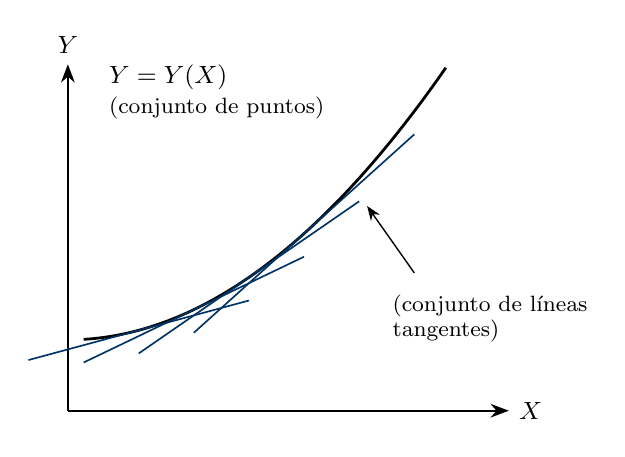
\begin{tikzpicture}
  \draw[ejes] (0,0) -- (5.6,0) node[right] {$X$};
  \draw[ejes] (0,0) -- (0,4.4) node[above] {$Y$};
  \draw[line width=1pt,domain=0.2:4.8,samples=50,smooth,variable=\x] plot ({\x},{0.15*\x*\x+0.9});
  \draw[line width=0.6pt,UGblue,domain=-0.4999999999999999:2.3,variable=\t] plot (\t,{1.0215+0.2700*(\t-0.9)});
  \draw[line width=0.6pt,UGblue,domain=0.20000000000000018:3.0,variable=\t] plot (\t,{1.2840+0.4800*(\t-1.6)});
  \draw[line width=0.6pt,UGblue,domain=0.8999999999999999:3.6999999999999997,variable=\t] plot (\t,{1.6935+0.6900*(\t-2.3)});
  \draw[line width=0.6pt,UGblue,domain=1.6:4.4,variable=\t] plot (\t,{2.2500+0.9000*(\t-3.0)});
  \node[right,align=left] at (0.4,4.05) {$Y=Y(X)$\\ {\footnotesize (conjunto de puntos)}};
  \node[below right,align=left] at (4.0,1.6) {\footnotesize (conjunto de líneas\\[-2pt] \footnotesize tangentes)};
  \draw[->,line width=0.5pt] (4.4,1.75) -- (3.8,2.6);
\end{tikzpicture}
\end{document}
